\chapter{Drift and Diffusion Current}
Total current flow is made up of drift current and diffusion current. If we apply an electric field $E$ to a semiconductor crystal, then holes accelerate in the direction of $E$ and free electrons accelerate in the opposite direction of $E$. While \textbf{drift current} is movement caused by electric fields, \textbf{diffusion current} is movement caused by variation in the carrier concentration. 

\section{Drift Current}
    \[v_{p-drift} = \mu_p E, ~~~~~ v_{n-drift} = - \mu_n E\]

\begin{gline}
    \item $E$: electric field, V/cm
    \item $v_{p-drift}$: drift velocity of holes, cm/s
    \item $v_{n-drift}$: drift velocity of electrons, cm/s
    \item $\mu_p$: hole mobility, cm\sq/V $\cdot$ s, 480 cm\sq/V $\cdot$ s for intrinsic silicon
    \item $\mu_n$: electron mobility, cm\sq/V $\cdot$ s, 1350 cm\sq/V $\cdot$ s for intrinsic silicon
\end{gline}

Current density is the current per unit cross-sectional area
    \[J_p = qn\mu_p E, ~~~~~ J_n = qn\mu_n E\]
Total drift current density is
    \[J = J_p + J_n = q(p\mu_p + n\mu_n) E = \sigma E\]
Via pattern matching, we can see that conductivity $\sigma$ is given by $\sigma = q(p\mu_p + n\mu_n)$ and resistivity is the inverse of this.

\section{Diffusion Current}
\textbf{Diffusion current} is the diffusion of charge carriers that give rose to a net flow of charge fro a region of high concentration to a region of low concentration. This implies that we can have current without voltage. We can write the current density as a function of the \textbf{concentration gradient} (slope of the concentration profile) at any point such that:
    \[J_p = -q D_p \frac{dp(x)}{dx}, ~~~~~ J_n = q D_n \frac{dn(X)}{dx}\]
\begin{gline}
    \item $J_p, J_n$: hole/electron-current density, A/cm\sq
    \item $q$: magnitude of the electron charge
    \item $D_p, D_n$: diffusion constant or diffusivity of holes/electrons. For intrinsic silicon, $D_p = 12$ cm\sq/s and $D_n = 35$ cm\sq/s
    \item $p(x), n(x)$: hole/electron concentration at point $x$. Note that if $\frac{dp(x)}{dx} < 0$, $J_p$ ends up being positive.
\end{gline}
This equation shows that current density is proportional to the slope of the concentration.
The image below shows a bar of silicon and an injection of holes on the left side, which will result in hole diffusion current in the same direct (positive direction of $x$)

\begin{figure}[H]
    \centering
    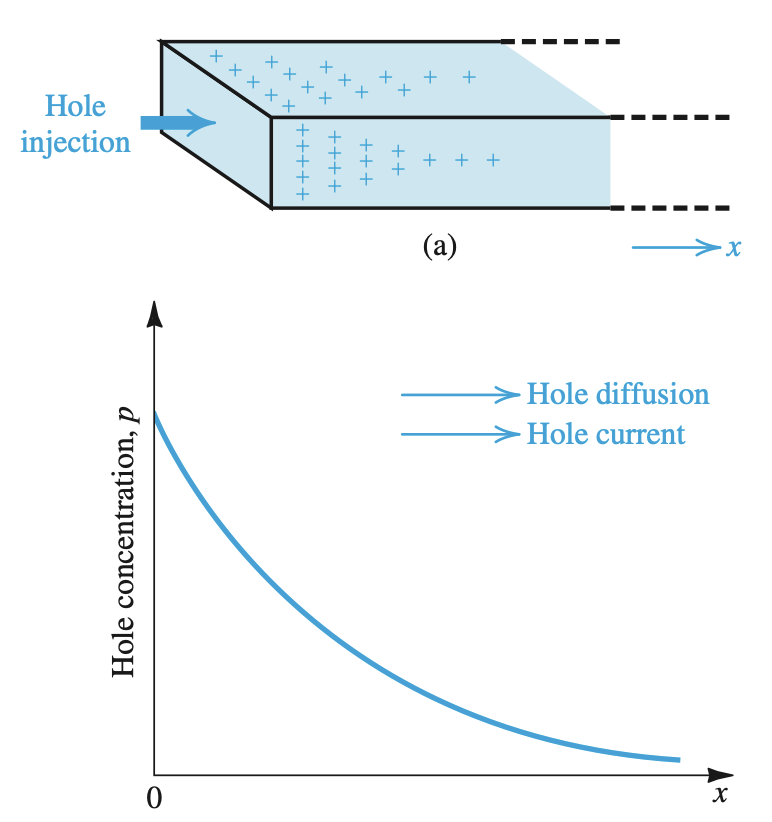
\includegraphics[scale=0.5]{figs/ch02/diffusion_current.png}
\end{figure}

Suppose we fill a gas chamber that is divided into two sections with a gases of temperature $T$ on one side. If we remove this divider, the gas will fill the entire volume of the new chamber. This occurs due to the concentration gradient. If the gas molecules here were charged, there would be a net current flow.

\begin{Analysis}{Einstein Relationship}{}
    The following equation is known as the \textbf{Einstein relationship}:
        \[\frac{D_n}{\mu_n} = \frac{D_p}{\mu_p} = V_T = \frac{kT}{q}\]
    \begin{gline}
        \item $V_T$: thermal voltage; at $T \simeq 300$ K, $V_T = 25.9$ mV
    \end{gline}
    We see that the diffusion constant is related to the mobility.
\end{Analysis}
Total current will be given by the sum of drift and diffusion currents. In resistors, since the carrier is approximately uniform, diffusion current is nearly zero.
    \[J^n = J_{drift}^n + J_{diff}^n = q\mu_n n E + qD_n \frac{dn}{dx}\]

\section{Practice Problems}
\begin{enumerate}
    \item A uniform bar of $n$-type silicon of 2-$\mu$m length has a voltage of 1 V applied across it. If $N_D = 10^{16}$ \conc and $\mu_n = 1350$ cm\sq/V $\cdot$ s, find (a) the electron drift velocity, (b) the time it takes an electron to cross the 2-$\mu$m length, (c) the drift-current density, and the (d) drift current in the case that the silicon bar has a cross-sectional area of 0.25 \mun\sq.
    \begin{Ans}
        \begin{todo}
           \item TODO: finish out this question
        \end{todo}
    \end{Ans}

    \item A general relationship for the current density carried out by holes of density $p$ is $J = qpv$, where $q$ is the electronic charge and $v$ is the hole velocity.
    \begin{enumerate}
        \item Find the velocity of holes, $v(x)$, that are moving only by diffusion if they have a density distribution of $p(x) = p_0 e^{-x/l}$ . The electric field is zero.
        \item What would be the electric field that would lead to a hole drift velocity equal to that of the diffusion velocity in part(a)? Use Einstein's relation to answer this question.
        \item At 300 K, what is the value of $l$ to make the ecltric field in part (b) be 1000 V/cm?
    \end{enumerate}
\end{enumerate}

\section{Sources}
\begin{itemize}
    % \item \href{https://www.youtube.com/watch?v=NWolpDgi6_Y}{\textcolor{blue}{Razavi Electronics 1, Lec 2. Doping, Drift}}
    \item Sedra, Adel S., et al. Microelectronic Circuits. Oxford University Press, 2021
    \item \href{https://file.notion.so/f/f/048d6522-202b-48d4-b5d9-bc005bd602e2/214bf1f0-292f-48d6-9016-737d9f5da155/ee105_reader_v3.pdf?id=237a4300-3dbe-47d1-888b-ffae90d8352b&table=block&spaceId=048d6522-202b-48d4-b5d9-bc005bd602e2&expirationTimestamp=1714435200000&signature=yx-H1qvZJIodPfazOpwXX0Ce2mWMG8skOHl45xoPxus&downloadName=ee105_reader_v3.pdf}{EE105 Reader}
    \item Q2 fro here is Q2 from EE105 HW6
\end{itemize}